\subsection{Linux kernel sources}

\begin{frame}
  \frametitle{Location of the official kernel sources}
  \begin{itemize}
  \item The mainline versions of the Linux kernel, as released by Torvalds
    \begin{itemize}
    \item These versions follow the development model of the kernel
    \item They may not contain the latest developments from a specific
      area yet
    \item A good pick for products development phase
    \item \url{https://git.kernel.org/pub/scm/linux/kernel/git/torvalds/linux.git}
    \end{itemize}
  \end{itemize}
\end{frame}

\begin{frame}
  \frametitle{Linux versioning scheme}
  \begin{itemize}
  \item Until 2003, there was a new ``stabilized'' release branch of Linux every
        2 or 3 years (2.0, 2.2, 2.4). Development branches took 2-3
        years to be merged (too slow!).
  \item Since 2003, there is a new official release of Linux about every
	10 weeks:
  \begin{itemize}
	\item Versions \code{2.6} (Dec. 2003) to \code{2.6.39} (May 2011)
	\item Versions \code{3.0} (Jul. 2011) to \code{3.19} (Feb. 2015)
	\item Versions \code{4.0} (Apr. 2015) to \code{4.20} (Dec. 2018)
	\item Versions \code{5.0} (Mar. 2019) to \code{5.19} (July 2022)
	\item Version \code{6.0} was released in Oct. 2022.
  \end{itemize}
  \item Features are added to the kernel in a progressive way. Since
        2003, kernel developers have managed to do so without having
        to introduce a massively incompatible development branch.
  \end{itemize}
\end{frame}

\begin{frame}
  \frametitle{Linux development model}
  \begin{itemize}
  \item Each new release starts with a two-week merge window for new
    features
  \item Follow about 8 release candidates (one week each)
  \item Until adoption of a new official release.
  \end{itemize}
  \begin{center}
    \includegraphics[width=0.8\textwidth]{slides/kernel-intro-sources/development-process-simple.pdf}
  \end{center}
\end{frame}

\begin{frame}[fragile]
  \frametitle{Need to further stabilize the official kernels}
  \begin{itemize}
  \item Issue: bug and security fixes only merged into the master
    branch, need to update to the latest kernel to benefit from them.
  \item Solution: a stable maintainers team goes through all the patches
    merged into Torvald's tree and backports the relevant ones into
    their stable branches for at least a few monthes.
  \end{itemize}
  \begin{center}
    \includegraphics[width=0.65\textwidth]{slides/kernel-intro-sources/development-process.pdf}
  \end{center}
\end{frame}

\begin{frame}
  \frametitle{Location of the stable kernel sources}
  \begin{itemize}
    \item The stable versions of the Linux kernel, as maintained by a
      maintainers group
    \begin{itemize}
    \item These versions do not bring new features compared to Linus'
      tree
    \item Only bug fixes and security fixes are pulled there
    \item Each version is stabilized during the development period of
      the next mainline kernel
    \item A good pick for products commercialization phase
    \item \url{https://git.kernel.org/pub/scm/linux/kernel/git/stable/linux.git}
    \item Certain versions will be maintained much longer
    \end{itemize}
  \end{itemize}
\end{frame}

\begin{frame}[fragile]
  \frametitle{Need for long term support}
  \begin{itemize}
  \item Issue: bug and security fixes only released for most recent
    kernel versions.
  \item Solution: the last release of each year is made an LTS {\em (Long Term
     Support)} release, and is supposed to be supported (and receive bug
    and security fixes) for up to 6 years.
  \begin{columns}
  \column{0.6\textwidth}
  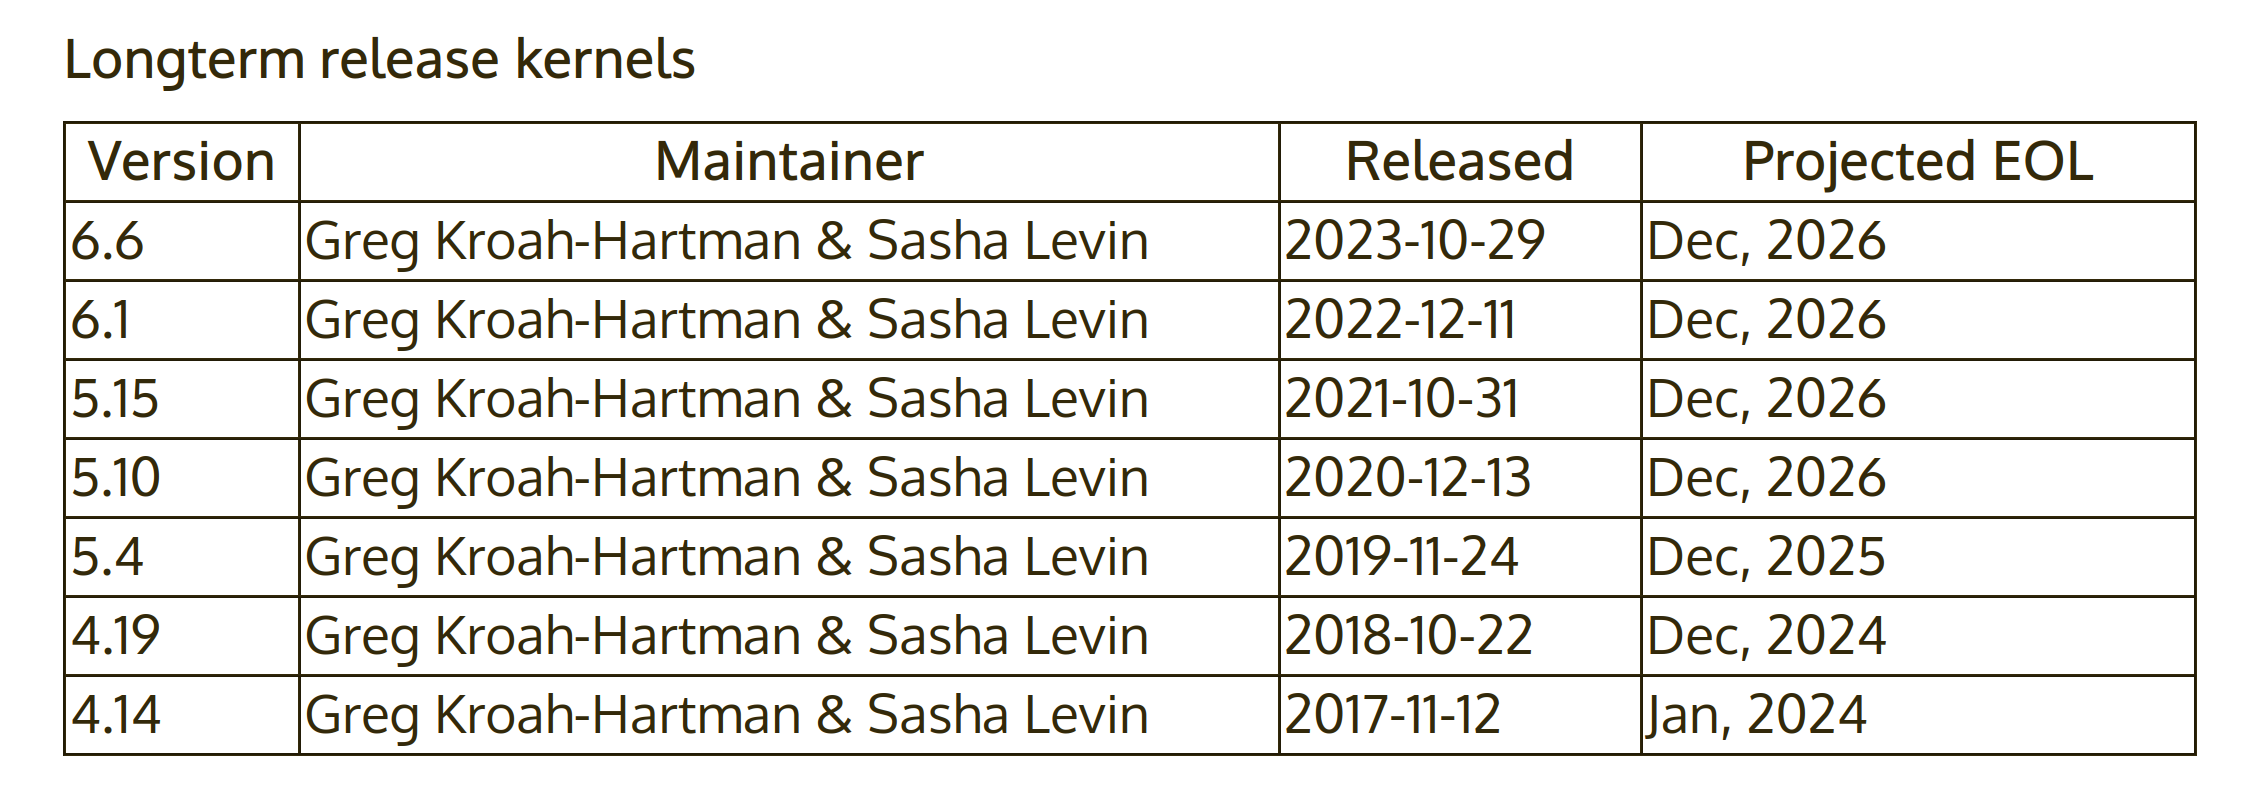
\includegraphics[width=\textwidth]{common/long-term-support-kernels.png}\\
  \column{0.4\textwidth}
  \scriptsize
   Captured on \url{https://kernel.org} in Apr. 2023, following the
   \href{https://www.kernel.org/category/releases.html}{\em Releases} link.
  \end{columns}
  \item Example at Google: starting from {\em Android O (2017)}, all new Android devices will
    have to run such an LTS kernel.
  \end{itemize}
\end{frame}

\begin{frame}[fragile]
  \frametitle{Need for even longer term support}
  \begin{itemize}
  \item You could also get long term support from a commercial embedded
    Linux provider.
    \begin{itemize}
	\item Wind River Linux can be supported for up to 15 years.
	\item Ubuntu Core can be supported for up to 10 years.
    \end{itemize}
  \item {\em "If you are not using a supported distribution kernel, or a stable / longterm
    kernel, you have an insecure kernel"} - Greg KH, 2019\\
    Some vulnerabilities are fixed in stable without ever getting a CVE.
  \item The {\em Civil Infrastructure Platform} project is an industry /
    Linux Foundation effort to support much longer (at least 10 years)
    selected LTS versions (currently 4.4, 4.19, 5.10) on selected architectures.
    See \url{https://wiki.linuxfoundation.org/civilinfrastructureplatform/cipkernelmaintenance}.
  \end{itemize}
\end{frame}

\begin{frame}
  \frametitle{Location of non-official kernel sources}
  \begin{itemize}
  \item Many chip vendors supply their own kernel sources
    \begin{itemize}
    \item Focusing on hardware support first
    \item Can have a very important delta with mainline Linux
    \item Sometimes they break support for other platforms/devices
      without caring
    \item Useful in early phases only when mainline hasn't caught up yet
      (many vendors invest in the mainline kernel at the same time)
    \item Suitable for PoC, not suitable for products on the long term
      as usually no updates are provided to these kernels
    \item Getting stuck with a deprecated system with broken software
      that cannot be updated has a real cost in the end
    \end{itemize}
  \item Many kernel sub-communities maintain their own kernel, with
    usually newer but fewer stable features, only for cutting-edge
    development
    \begin{itemize}
    \item Architecture communities (ARM, MIPS, PowerPC, etc)
    \item Device drivers communities (I2C, SPI, USB, PCI, network, etc)
    \item Other communities (real-time, etc)
    \item Not suitable to be used in products
    \end{itemize}
  \end{itemize}
\end{frame}

\begin{frame}
  \frametitle{Linux kernel size and structure}
  \begin{itemize}
  \item Linux v5.18 sources: close to 80k files, 35M lines, 1.3GiB
    % files: git ls-files | wc -l
    % lines: git ls-files | xargs cat | wc -l
    % bytes: git ls-files | xargs cat | wc -c
  \item But a compressed Linux kernel just sizes a few megabytes.
  \item So, why are these sources so big?\\
    Because they include numerous device drivers, network protocols,
    architectures, filesystems... The core is pretty small!
  \item As of kernel version v5.18 (in percentage of total number of lines):
  % Update the data by running utils/source-code-line-statistics
  % in the Linux kernel source directory
  \end{itemize}
  {\small
  \begin{columns}
    \column[t]{0.24\textwidth}
    \begin{itemize}
    \item \kdir{drivers}: 61.1\%
    \item \kdir{arch}: 11.6\%
    \item \kdir{fs}: 4.4\%
    \item \kdir{sound}: 4.1\%
    \item \kdir{tools}: 3.9\%
    \item \kdir{net}: 3.7\%
    \end{itemize}
    \column[t]{0.30\textwidth}
    \begin{itemize}
    \item \kdir{include}: 3.5\%
    \item \kdir{Documentation}: 3.4\%
    \item \kdir{kernel}: 1.3\%
    \item \kdir{lib}: 0.7\%
    \item \kdir{usr}: 0.6\%
    \item \kdir{mm}: 0.5\%
    \end{itemize}
    \column[t]{0.40\textwidth}
    \begin{itemize}
    \item \kdir{scripts}, \kdir{security}, \kdir{crypto}, \kdir{block},
      \kdir{samples}, \kdir{ipc}, \kdir{virt}, \kdir{init}, \kdir{certs}: <0.5\%
    \item Build system files: \kfile{Kbuild}, \kfile{Kconfig}, \kfile{Makefile}
    \item Other files: \kfile{COPYING}, \kfile{CREDITS},
      \kfile{MAINTAINERS}, \kfile{README}
    \end{itemize}
  \end{columns}
  }
\end{frame}
